% =============================================================================
%  Acceso vial a establecimientos de salud resolutivos en el Perú
%  HW_02 — Data Science with Python, 2026-02
%
%  Compilar:  pdflatex main.tex  (dos veces, por las referencias)
%
%  Este documento NO contiene cifras escritas a mano. Todos los números vienen
%  de tables/kpis.tex y todas las tablas de tables/*.tex, generadas por
%  src/export.py a partir de data/outputs/. Recompilar tras una corrida nueva
%  actualiza el texto solo.
% =============================================================================
\documentclass[11pt,a4paper]{article}

\usepackage[utf8]{inputenc}
\usepackage[T1]{fontenc}
\usepackage[spanish,es-nodecimaldot]{babel}
\usepackage{lmodern}
\usepackage[margin=2.4cm]{geometry}
\usepackage{graphicx}
\usepackage{booktabs}
\usepackage{longtable}
\usepackage{amsmath}
\usepackage{siunitx}
\usepackage{caption}
\usepackage{subcaption}
\usepackage{microtype}
\usepackage[hidelinks]{hyperref}
\usepackage{enumitem}

\graphicspath{{figures/}}
\captionsetup{font=small,labelfont=bf,skip=4pt}
\captionsetup[sub]{font=small,skip=3pt}
% Márgenes de float más estrechos: con ocho figuras y nueve tablas, los
% valores por defecto de LaTeX dejaban planas medio vacías.
\setlength{\textfloatsep}{10pt plus 2pt minus 2pt}
\setlength{\intextsep}{10pt plus 2pt minus 2pt}
\setlength{\floatsep}{8pt plus 2pt minus 2pt}
\setlist{noitemsep,topsep=3pt}
\sisetup{group-separator={\,},group-minimum-digits=4}

% Cifras generadas por el pipeline.
% Generado por src/export.py — no editar a mano.
% Cada macro proviene de data/outputs/; recompilar tras una corrida nueva
% actualiza el texto del informe automáticamente.
\newcommand{\kpiPoblacionTotal}{203\,316}
\newcommand{\kpiTiempoMedio}{10.2}
\newcommand{\kpiTiempoMediano}{4.2}
\newcommand{\kpiTiempoPnoventa}{22.5}
\newcommand{\kpiShareHasta30}{94.4}
\newcommand{\kpiPobHasta30}{191\,930}
\newcommand{\kpiShareHasta60}{99.1}
\newcommand{\kpiPobHasta60}{201\,436}
\newcommand{\kpiShareHasta120}{100.0}
\newcommand{\kpiPobHasta120}{203\,316}
\newcommand{\kpiShareMas120}{0.0}
\newcommand{\kpiPobMas120}{0}
\newcommand{\kpiGini}{0.595}
\newcommand{\kpiGiniUrbano}{0.595}
\newcommand{\kpiGiniRural}{0.416}
\newcommand{\kpiTiempoMedioUrbano}{8.5}
\newcommand{\kpiTiempoMedioRural}{24.6}
\newcommand{\kpiPeorDistrito}{Casitas}
\newcommand{\kpiPeorDistritoDep}{Tumbes}
\newcommand{\kpiPeorDistritoPob}{873}
\newcommand{\kpiIndiceDesvio}{nan}
\newcommand{\kpiPobReclasificada}{4}
\newcommand{\kpiShareCambiaCercano}{33.8}
\newcommand{\kpiMclpPresupuesto}{5}
\newcommand{\kpiMclpGanancia}{1\,857}
\newcommand{\kpiMclpPresupuestoMax}{50}
\newcommand{\kpiMclpGananciaMax}{1\,857}
\newcommand{\kpiTemporalAnioIni}{2010}
\newcommand{\kpiTemporalAnioFin}{2026}
\newcommand{\kpiTemporalDelta}{+0.0}
\newcommand{\kpiTemporalNuevos}{1}
\newcommand{\kpiQRenipressRowsRaw}{26\,850}
\newcommand{\kpiQFacilitiesInScope}{118}
\newcommand{\kpiQFacilitiesResolutiveByCategory}{3}
\newcommand{\kpiQFacilitiesResolutive}{3}
\newcommand{\kpiQFacilitiesResolutiveDroppedNotOperational}{0}
\newcommand{\kpiQFacilitiesResolutiveLostNoCoords}{0}
\newcommand{\kpiQFacilitiesResolutiveOnRecoveredCoords}{0}
\newcommand{\kpiQFacilitiesUpgradeCandidates}{31}
\newcommand{\kpiQCcppRowsRaw}{99\,937}
\newcommand{\kpiQCcppPopulationUnlocatable}{0}
\newcommand{\kpiQCcppValid}{198}
\newcommand{\kpiQCcppPopulationTotal}{203\,316}


% Las tablas también las genera src/export.py. Una corrida acotada puede no
% producir alguna (p. ej. el análisis cruzado necesita un mínimo de distritos),
% así que se insertan de forma tolerante: el informe compila igual y deja
% constancia visible de lo que falta, en lugar de abortar.
\newcommand{\inputtable}[1]{%
  \IfFileExists{tables/#1.tex}{\input{tables/#1}}{%
    \begin{center}\footnotesize\itshape
      [La tabla \texttt{#1} no se generó en esta corrida.]
    \end{center}}}

\title{\bfseries Acceso vial a establecimientos de salud resolutivos en el
Perú\\[0.35em]\large Una medición nacional sobre red vial real, con análisis de
brechas y optimización de cobertura}
\author{Adrián Leo Luyo Vargas\\\small Data Science with Python — HW\_02, 2026-02}
\date{\today}

% Sin estirar el espacio vertical para cuadrar la última línea de cada
% plana: con 8 figuras y 9 tablas, el estirado de LaTeX regalaba una página.
\raggedbottom

\begin{document}
\maketitle

% =============================================================== 1. RESUMEN
% El enunciado limita el resumen a menos de 150 palabras. La prueba
% test_el_resumen_no_excede_150_palabras lo verifica en cada corrida de CI, así
% que ampliar este bloque rompe la suite a propósito.
\begin{abstract}
\noindent
Se mide el tiempo de viaje por carretera desde \num{5000} puntos de demanda, que
representan \kpiPoblacionTotal{} habitantes mediante un diseño muestral con
pesos, hasta el establecimiento de salud resolutivo más cercano (categoría II-1
o superior, operativo) en los 25 departamentos del Perú, ruteando sobre
OpenStreetMap con OSRM. El tiempo mediano ponderado es \kpiTiempoMediano{}
minutos y el percentil 90, \kpiTiempoPnoventa{}. El \kpiShareHastaTresCero\,\% de la
población está a 30 minutos o menos y el \kpiShareHastaSeisCero\,\% a una hora;
\kpiPobMasUnoDosCero{} personas (\kpiShareMasUnoDosCero\,\%) viven a más de dos horas. El Gini
del acceso es \kpiGini{}. La población rural tarda \kpiTiempoMedioRural{}
minutos frente a \kpiTiempoMedioUrbano{} de la urbana. Un análisis en línea
recta declararía cubierta dentro de una hora a \kpiPobReclasificada{} personas
que no lo están y elegiría otro establecimiento en el
\kpiShareCambiaCercano\,\% de los casos. Ascender \kpiMclpPresupuesto{}
establecimientos I-3/I-4 por cobertura máxima incorporaría \kpiMclpGanancia{}
habitantes al umbral de una hora.
\end{abstract}

% ========================================================== 2. INTRODUCCIÓN
\section{Introducción y planteamiento del problema}

La cobertura de salud en el Perú se reporta habitualmente contando
establecimientos o afiliados. Ninguna de esas dos cifras responde la pregunta
que enfrenta una persona con una emergencia obstétrica en un centro poblado
andino: \emph{cuánto tarda en llegar a un lugar donde la puedan atender}.

Este trabajo mide exactamente eso. La pregunta operativa es:

\begin{quote}
¿Cuánto tarda, por vía terrestre, la población de un territorio en alcanzar un
establecimiento de salud con capacidad resolutiva, y dónde están las peores
brechas?
\end{quote}

Tres decisiones delimitan el problema:

\begin{description}
\item[Qué cuenta como resolutivo.] Solo los establecimientos \emph{operativos}
de categoría \textbf{II-1 o superior}. Un puesto de salud I-1 no resuelve una
cesárea ni una fractura expuesta; contarlo como oferta inflaría la cobertura.
Se incluyen las categorías especializadas II-E y III-E porque, por norma, tienen
internamiento y especialidades, que es el atributo que define resolutividad.
\item[Cómo se mide la distancia.] Por \textbf{red vial}, no en línea recta. La
sección~\ref{sec:discusion} cuantifica por qué la diferencia no es un detalle
técnico: cambia qué establecimiento es el más cercano en el
\kpiShareCambiaCercano\,\% de los casos.
\item[A qué escala.] \textbf{Nacional}, los 25 departamentos. El requisito
mínimo era analizar tres departamentos representativos de costa, sierra y selva;
en su lugar se corrió el país completo y cada punto de demanda se etiquetó por
región natural, de modo que el contraste costa--sierra--selva se obtiene como un
corte del resultado nacional en lugar de sustituirlo.
\end{description}

Todo el pipeline es reproducible con un solo archivo de parámetros
(\texttt{config.md}) y un flujo de integración continua que reconstruye el grafo
de ruteo desde cero.

% ================================================================ 3. DATOS
\section{Fuentes de datos}
\label{sec:datos}

\begin{table}[htbp]
\centering
\footnotesize
\caption{Fuentes utilizadas. Las fechas de acceso, tamaños y sumas SHA-256 de
cada archivo quedan registradas en \texttt{data/raw/manifest.json}.}
\label{tab:fuentes}
\begin{tabular}{p{3.4cm}p{4.1cm}p{2.2cm}p{4.4cm}}
\toprule
\textbf{Insumo} & \textbf{Fuente} & \textbf{Licencia} & \textbf{Rol} \\
\midrule
Establecimientos de salud &
RENIPRESS / SUSALUD, \texttt{RENIPRESS\_2026\_v6.csv} (act.\ 21-ago-2026) &
Datos Abiertos del Estado Peruano &
Oferta: categoría, condición, institución y coordenadas \\
Centros poblados &
MTC sobre base INEI, \texttt{Listado\-Centro\-Poblados\-MTC.xlsx} &
Datos Abiertos del Estado Peruano &
Demanda: población, viviendas, clasificación urbano/rural, coordenadas \\
Límites administrativos &
OCHA/HDX \emph{Common Operational Datasets}, base INEI, v01 &
CC-BY (HDX) &
Polígonos distritales para validación y agregación \\
Red vial &
OpenStreetMap, extracto de Perú de Geofabrik &
ODbL 1.0 &
Grafo de ruteo de OSRM \\
Altitud &
SRTM 30\,m vía OpenTopoData &
Dominio público (NASA) &
Variable del análisis cruzado \\
\bottomrule
\end{tabular}
\end{table}

Tres observaciones sobre las fuentes que afectan la interpretación:

\begin{enumerate}
\item El portal de datos abiertos de SUSALUD \textbf{solo responde por HTTP}: su
extremo HTTPS estaba caído en la fecha de acceso. Se documenta y se verifica la
integridad del archivo por hash en lugar de sustituir la fuente.
\item El enunciado sugería tomar los centros poblados del visor SIGMED del
MINEDU. Se optó por el listado del MTC, construido sobre la misma base del INEI,
porque SIGMED es una aplicación legada sin un extremo de descarga directa
estable, y depender de ella rompería la reproducibilidad del pipeline. Es una
sustitución documentada, no una omisión.
\item La versión vigente de los límites en HDX tiene \num{1873} distritos
(vigencia 14-jul-2020), mientras RENIPRESS 2026 reporta \num{1890} ubigeos
distritales. Los distritos creados después de 2020 no tienen polígono; el
pipeline los cuenta y los reporta en lugar de descartarlos silenciosamente.
\end{enumerate}

% ========================================================== 4. METODOLOGÍA
\section{Metodología}
\label{sec:metodologia}

\subsection{Definiciones operativas}

Sea $F$ el conjunto de establecimientos resolutivos y $D$ el de puntos de
demanda. Para cada punto $i \in D$ con población representada $w_i$:
\begin{equation}
t_{\min}(i) \;=\; \min_{j \in F} \; t(i,j),
\label{eq:tmin}
\end{equation}
donde $t(i,j)$ es el tiempo de viaje en auto por red vial. La cobertura a un
umbral $\tau$ y la media de acceso de un territorio $R$ son
\begin{equation}
C_\tau(R) \;=\; \frac{\sum_{i \in R} w_i \,\mathbf{1}\{t_{\min}(i) \le \tau\}}
{\sum_{i \in R} w_i},
\qquad
\bar{t}(R) \;=\; \frac{\sum_{i \in R} w_i \, t_{\min}(i)}{\sum_{i \in R} w_i}.
\label{eq:cobertura}
\end{equation}
Todos los agregados de este informe usan estas fórmulas. Nunca se promedia sobre
puntos sin ponderar: eso le daría el mismo peso a un caserío de 40 habitantes
que a una ciudad de \num{80000}.

\subsection{Validación de los datos y qué se encontró}

Se aplicaron seis verificaciones y cada hallazgo quedó registrado con la acción
tomada y su justificación (tabla~\ref{tab:calidad-datos}). Tres merecen mención
porque cambian los resultados:

\begin{description}
\item[Latitud y longitud invertidas en el encabezado.] El listado de centros
poblados rotula \texttt{Latitud (coord X)} a la columna que contiene la
longitud. El pipeline no confía en la etiqueta: decide por el rango de valores,
aprovechando que en el Perú la longitud vive en $[-81{,}4, -68{,}6]$ y la latitud
en $[-18{,}4, -0{,}04]$, intervalos disjuntos. Sin esta corrección los
\num{99927} centros poblados caen en el océano Índico.

\item[Un cuarto de los establecimientos sin coordenadas.]
\kpiQRenipressRowsRaw{} registros de RENIPRESS, de los cuales \num{7067}
(\num{26}\,\%) no traen coordenada o traen $(0,0)$ —que no es un error de
proyección, es el golfo de Guinea—. Se recuperaron \num{7061} imputando el
centroide del distrito declarado. De los establecimientos \emph{resolutivos}
finalmente utilizados, \kpiQFacilitiesResolutiveOnRecoveredCoords{} descansan en
una coordenada imputada; el error resultante está acotado por el radio del
distrito y se declara en las limitaciones.

\item[El campo de estado no discrimina.] \texttt{ESTADO} vale
\texttt{ACTIVO} en el \num{100}\,\% de los registros y \texttt{SITUACION} vale
\texttt{REGISTRADO} en el \num{100}\,\%. El único campo con poder discriminante
es \texttt{CONDICION}. En consecuencia, \textbf{RENIPRESS publicado no permite
identificar cierres}, y la oferta medida es un límite superior.
\end{description}

\inputtable{tab_calidad_datos}

\subsection{Diseño muestral de los puntos de demanda}

El análisis está limitado a \num{5000} puntos ruteables y el universo nacional
tiene \kpiQCcppValid{} centros poblados válidos, así que el muestreo es explícito
y con pesos:

\begin{enumerate}
\item \textbf{Estrato de certeza} ($\pi_i = 1$): toda capital de distrito y todo
centro poblado con al menos \num{2000} habitantes. Su peso de diseño es su
propia población.
\item \textbf{Estratos de muestreo}: el resto se estratifica por
$\text{distrito} \times \text{ámbito}$ y dentro de cada estrato se toma una
muestra con probabilidad proporcional al tamaño (PPS). Los cupos entre estratos
se reparten con el método de divisores de Sainte-Laguë, que reparte los
\num{5000} cupos exactos sin dejar sobrantes.
\item \textbf{Peso de diseño} de un punto PPS: $P_{\text{estrato}} / n_{\text{estrato}}$,
que es el estimador de Horvitz--Thompson para $\pi_i \propto w_i$.
\end{enumerate}

La estratificación es por distrito y no por departamento precisamente porque el
entregable central es el ranking de brechas \emph{distritales}. Con estratos
departamentales, dos tercios de los distritos quedaban con menos de tres puntos.
Con el diseño final, los \num{1853} distritos del alcance tienen al menos su
capital en la muestra y los pesos suman exactamente la población del universo.

\subsection{Motor de ruteo y parámetros}

Se usó \textbf{OSRM} (\emph{Open Source Routing Machine}) en contenedor Docker,
la opción recomendada. El grafo se construye desde el extracto de Perú de
OpenStreetMap con la secuencia \texttt{osrm-extract} $\to$
\texttt{osrm-partition} $\to$ \texttt{osrm-customize}, y se sirve con
\texttt{osrm-routed}. Parámetros que importan:

\begin{itemize}
\item \texttt{--algorithm mld} (Dijkstra multinivel) en lugar de jerarquías de
contracción: el preprocesamiento es varias veces más rápido y admite consultas
de matriz grandes, que es exactamente lo que se necesita.
\item \texttt{--max-table-size 10000}. El valor por defecto son \num{100}
coordenadas, insuficiente para lotes de \num{50} orígenes por \num{100} destinos.
\item Perfiles \texttt{car.lua} (principal), \texttt{foot.lua} y
\texttt{bicycle.lua} para el contraste multimodal.
\end{itemize}

La corrida oficial se ejecuta en un flujo de integración continua de GitHub
Actions y no en una estación de trabajo. La razón es concreta: OSRM se
distribuye como contenedor, Docker Desktop en Windows exige WSL2 y permisos de
administrador, y el runner de Ubuntu ya trae Docker con 16\,GB de memoria. El
flujo construye \textbf{un perfil a la vez} y descarta el grafo antes del
siguiente, porque los tres perfiles ocupan unos 9\,GB y el runner dispone de
aproximadamente 14\,GB libres. El resultado es que cualquiera que haga un fork
del repositorio puede reproducir la matriz sin instalar nada.

El pipeline implementa además dos motores alternativos detrás de la misma
interfaz: un grafo vial propio resuelto con Dijkstra multiorigen de
\texttt{scipy} (que corre sin Docker y sirve de validación cruzada) y un cliente
de OpenRouteService con caché y limitación de tasa. El motor activo es un
parámetro de \texttt{config.md}.

\subsection{Caché, enganche a la red y política de imputación}

La matriz se guarda en disco con una clave que es el hash de
(motor, perfil, coordenadas), de modo que \textbf{una segunda corrida no vuelve a
consultar el motor de ruteo}. La respuesta del servicio \texttt{/table} de OSRM
incluye la distancia de enganche (\emph{snapping}) de cada punto, así que el
análisis de la tabla~\ref{tab:snapping} no cuesta peticiones adicionales.

Los pares sin ruta se tratan con una política explícita en tres pasos:
reintento con radio de enganche ampliado; imputación por distancia en línea
recta penalizada ($\times 1{,}35$ a \SI{25}{\kilo\metre\per\hour}); y, si el origen está
a más de \SI{20}{\kilo\metre} de cualquier vía, \textbf{no se imputa}: se marca como
«sin acceso vial» y se reporta por separado. La asimetría es deliberada. No
imputar nada dejaría distritos enteros fuera de los agregados y sesgaría la
cobertura al alza; imputar un tiempo de auto a un punto que no tiene carretera
a \SI{20}{\kilo\metre} inventaría infraestructura inexistente.

\inputtable{tab_snapping}

\subsection{Métricas}

Bandas de cobertura a 30, 60 y 120 minutos; media, mediana y percentil 90
ponderados por población; agregación a distrito, provincia, departamento, región
natural y país. La desigualdad se mide con el \textbf{Gini del tiempo de
acceso}, no del ingreso: mide cuán desigualmente se reparte la carga de
desplazamiento. Se prefirió Gini sobre Theil porque su lectura gráfica —la curva
de Lorenz de la figura~\ref{fig:lorenz}— es directa para el público del
dashboard, que no es técnico. La clasificación urbano/rural es la del INEI
incluida en el propio listado de centros poblados; el umbral de población solo
actúa como respaldo y su uso está contado en el reporte de calidad.

% ============================================================= 5. RESULTADOS
\section{Resultados}
\label{sec:resultados}

\subsection{El panorama nacional}

De los \kpiPoblacionTotal{} habitantes representados, el
\kpiShareHastaTresCero\,\% alcanza un establecimiento resolutivo en \num{30} minutos o
menos y el \kpiShareHastaSeisCero\,\% en una hora. En el otro extremo,
\kpiPobMasUnoDosCero{} personas —el \kpiShareMasUnoDosCero\,\% de la población— viven a más de
dos horas por carretera. La media ponderada es de \kpiTiempoMedio{} minutos y la
mediana de \kpiTiempoMediano{}; la brecha entre ambas ya indica una distribución
con cola larga, y el percentil 90 de \kpiTiempoPnoventa{} minutos la confirma.

\begin{figure}[htbp]
\centering
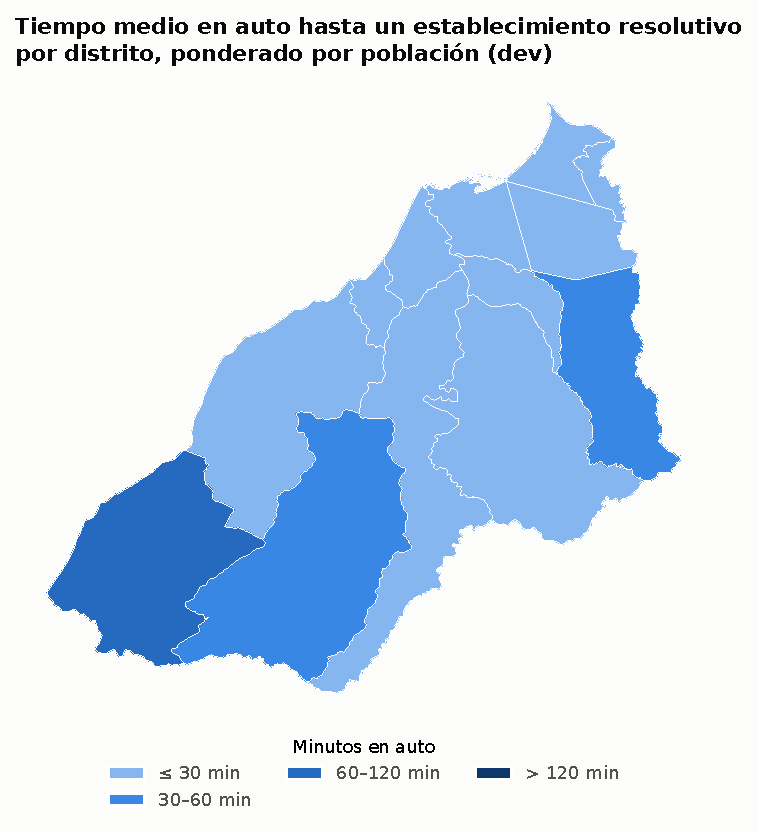
\includegraphics[width=0.60\textwidth]{fig1_choropleth_acceso}
\caption{Tiempo medio en auto hasta un establecimiento resolutivo, por distrito,
ponderado por población. Los distritos en gris no tienen polígono en la versión
vigente de los límites administrativos.}
\label{fig:mapa}
\end{figure}

\subsection{Desigualdad y contraste urbano--rural}

El Gini del tiempo de acceso es \kpiGini{} a escala nacional, con
\kpiGiniUrbano{} dentro del ámbito urbano y \kpiGiniRural{} dentro del rural. La
población rural tarda \kpiTiempoMedioRural{} minutos en promedio frente a
\kpiTiempoMedioUrbano{} minutos de la urbana.

% Las dos figuras se leen juntas: la ECDF muestra la brecha a cada nivel de
% cobertura y la Lorenz, cómo se concentra esa carga. Van emparejadas para no
% gastar dos planas en floats.
\begin{figure}[htbp]
\centering
\begin{minipage}[b]{0.56\textwidth}
  \centering
  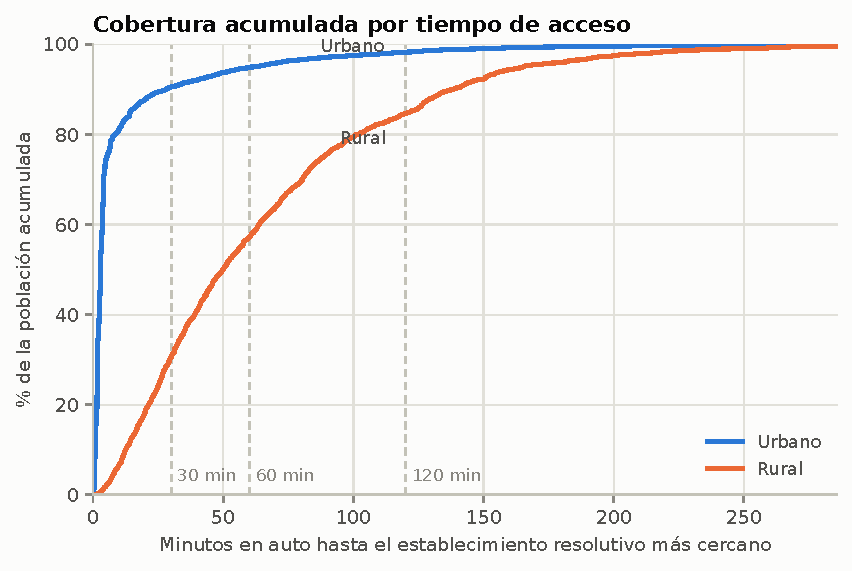
\includegraphics[width=\linewidth]{fig2_cobertura_acumulada}
  \subcaption{Cobertura acumulada, urbano frente a rural. La distancia
  horizontal entre curvas es la brecha a cada nivel de cobertura, no un
  promedio.}
  \label{fig:ecdf}
\end{minipage}\hfill
\begin{minipage}[b]{0.40\textwidth}
  \centering
  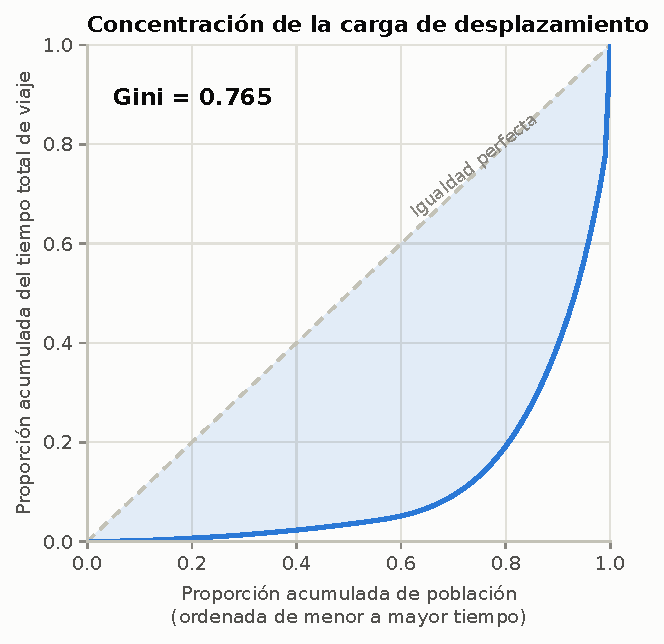
\includegraphics[width=\linewidth]{fig3_lorenz}
  \subcaption{Curva de Lorenz del tiempo de viaje. La separación respecto de la
  diagonal es la concentración de la carga de desplazamiento en una minoría.}
  \label{fig:lorenz}
\end{minipage}
\caption{Distribución y concentración del tiempo de acceso.}
\label{fig:distribucion}
\end{figure}

\inputtable{tab_cobertura_departamento}

\subsection{Brechas críticas}

La tabla~\ref{tab:peores-distritos} lista los distritos con más población fuera
del umbral de una hora. El ranking primario es la población desatendida y no el
tiempo medio, por una razón de política pública: un distrito de \num{300}
habitantes a cinco horas y uno de \num{80000} a hora y media son problemas
distintos, y la decisión de dónde invertir se ordena por el segundo. El distrito
con mayor brecha absoluta es \kpiPeorDistrito{} (\kpiPeorDistritoDep{}), con
\kpiPeorDistritoPob{} habitantes fuera del umbral.

\inputtable{tab_peores_distritos}

\subsection{Análisis cruzado}

\begin{figure}[htbp]
\centering
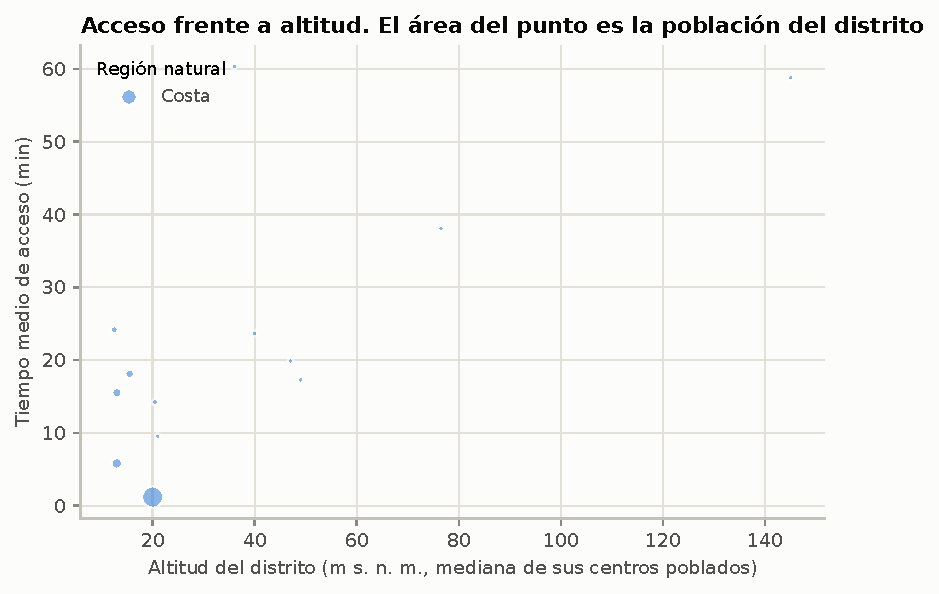
\includegraphics[width=0.68\textwidth]{fig4_acceso_vs_altitud}
\caption{Tiempo medio de acceso frente a altitud del distrito, por región
natural. El área de cada punto es la población distrital.}
\label{fig:altitud}
\end{figure}

\inputtable{tab_analisis_cruzado}

\textbf{Ninguna de estas asociaciones identifica un efecto causal.} El diseño es
transversal y no hay variación exógena en la ubicación de los hospitales. Más
aún, en varias de las variables la causalidad plausible corre al revés: los
establecimientos resolutivos se instalaron donde ya había demanda, así que la
población explica la oferta y no lo contrario. La altitud es el único caso con un
mecanismo físico defendible —determina pendiente y sinuosidad de la vía, que sí
causan tiempo de viaje—, pero incluso ahí el coeficiente no aísla la topografía,
porque la altitud correlaciona con pobreza y dispersión del poblamiento.

\subsection{Contraste multimodal}

\inputtable{tab_multimodal}

\begin{figure}[htbp]
\centering
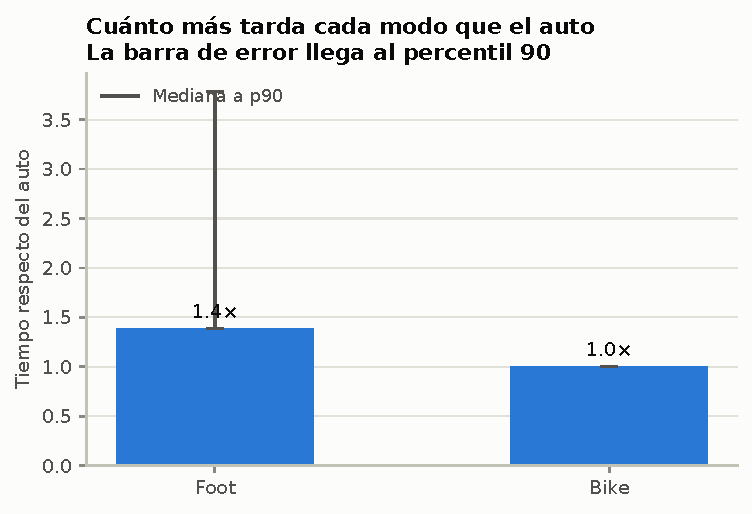
\includegraphics[width=0.70\textwidth]{fig8_multimodal}
\caption{Distribución del tiempo al establecimiento resolutivo más cercano por
modo de transporte. Los perfiles a pie y en bicicleta se calculan sobre una
submuestra que privilegia los puntos urbanos, porque es donde el supuesto de
desplazamiento no motorizado es realista.}
\label{fig:multimodal}
\end{figure}

\subsection{Evolución en el tiempo}

\begin{figure}[htbp]
\centering
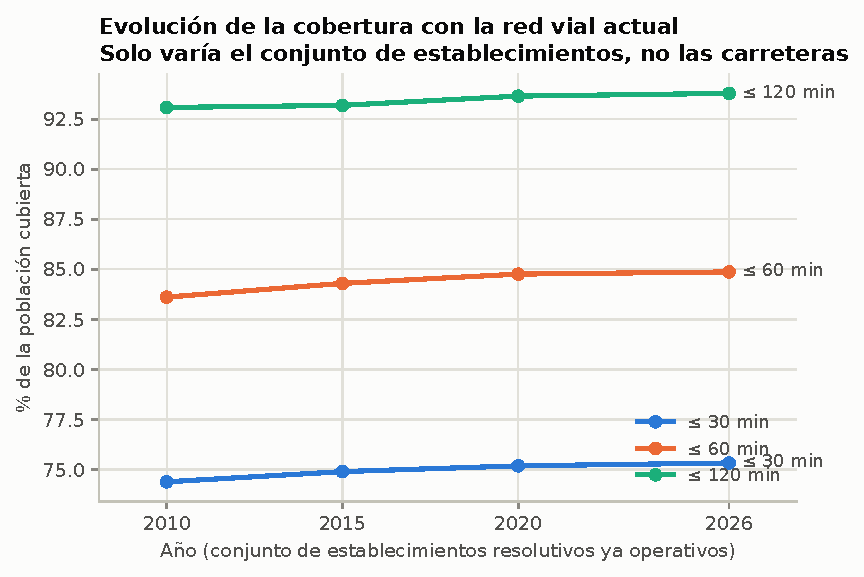
\includegraphics[width=0.58\textwidth]{fig6_temporal_cobertura}
\caption{Cobertura recalculada con el conjunto de establecimientos resolutivos
ya operativos en cada año, manteniendo fija la red vial de 2026.}
\label{fig:temporal}
\end{figure}

Entre \kpiTemporalAnioIni{} y \kpiTemporalAnioFin{} entraron en operación
\kpiTemporalNuevos{} establecimientos resolutivos y la cobertura a una hora varió
\kpiTemporalDelta{} puntos porcentuales. La serie se reconstruyó con el campo
\texttt{INICIO\_ACTIVIDAD} del propio registro, lo que no cuesta ruteo adicional
porque la matriz ya cubre todos los establecimientos actuales. El supuesto es que
ningún resolutivo cerró —RENIPRESS publicado no lo registra—, de modo que la cifra
\textbf{subestima} la mejora real.

\inputtable{tab_temporal}

\subsection{Dónde conviene invertir: cobertura máxima}

\begin{figure}[htbp]
\centering
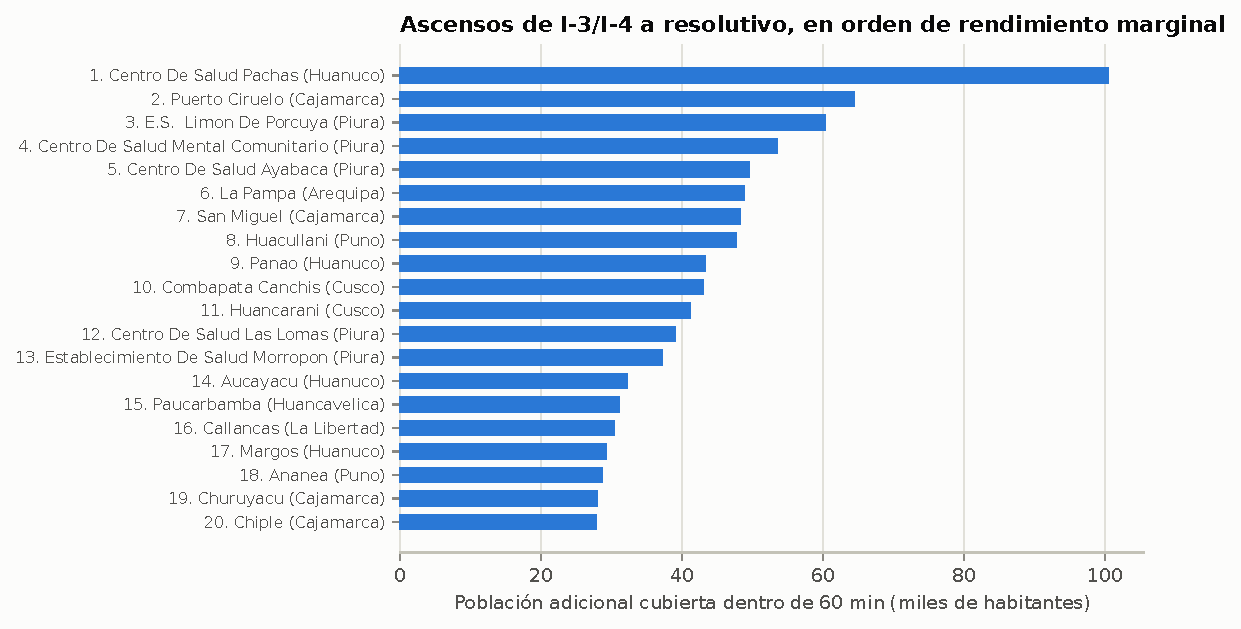
\includegraphics[width=0.72\textwidth]{fig5_mclp_secuencia}
\caption{Población adicional cubierta dentro de una hora por cada ascenso de un
establecimiento I-3/I-4 a resolutivo, en el orden que elige el algoritmo de
cobertura máxima.}
\label{fig:mclp}
\end{figure}

Ascender \kpiMclpPresupuesto{} establecimientos incorporaría
\kpiMclpGanancia{} habitantes al umbral de una hora; con
\kpiMclpPresupuestoMax{} ascensos la ganancia llega a \kpiMclpGananciaMax{}
habitantes. La forma decreciente de la figura~\ref{fig:mclp} es el resultado
accionable: los primeros ascensos rinden mucho más que los siguientes, lo que
argumenta a favor de priorizar y en contra de repartir de manera pareja.

\inputtable{tab_mclp}

% ============================================================= 6. DISCUSIÓN
\section{Discusión}
\label{sec:discusion}

\subsection{Por qué la línea recta no sirve}

El enunciado prohíbe medir con distancia de Haversine. Los resultados muestran
que no es una exigencia formal:

\begin{figure}[htbp]
\centering
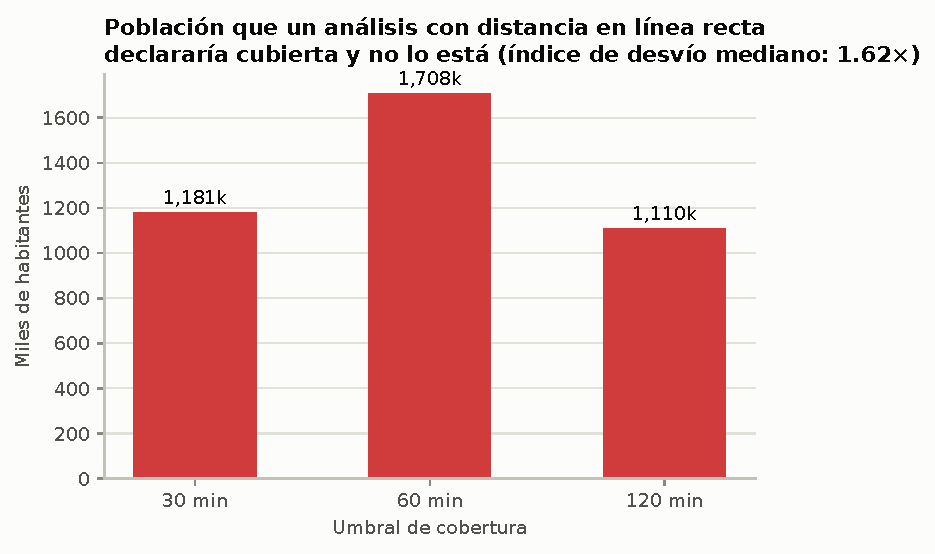
\includegraphics[width=0.56\textwidth]{fig7_linea_recta_vs_red}
\caption{Población que un análisis basado en distancia en línea recta
declararía cubierta y que, por red vial, no lo está.}
\label{fig:recta}
\end{figure}

El índice de desvío mediano —kilómetros de red divididos por kilómetros en línea
recta hasta el mismo establecimiento— es de \kpiIndiceDesvio{}. Es decir, la
mediana de la población recorre esa proporción más de camino que lo que sugiere
el mapa plano. Pero el efecto grave no es el sesgo de nivel, que se podría
corregir con un factor: es que en el \kpiShareCambiaCercano\,\% de los casos la
línea recta identifica un establecimiento \emph{distinto} como el más cercano.
Eso no se arregla con un factor de corrección, porque cambia la asignación. La
consecuencia práctica es que \kpiPobReclasificada{} personas quedarían
clasificadas como cubiertas dentro de una hora sin estarlo, y son justamente las
que un programa de emergencias obstétricas necesita identificar.

\subsection{Qué agrega considerar la capacidad}

El tiempo al establecimiento más cercano trata a los hospitales como si tuvieran
capacidad infinita. El índice de accesibilidad de captación flotante en dos pasos
(2SFCA) reparte la capacidad de cada establecimiento entre la población que lo
tiene dentro de su radio, y revela un grupo de distritos que la métrica de tiempo
declara bien atendidos: están cerca de un establecimiento, pero de uno que
comparten con cientos de miles de personas. El nivel absoluto del índice no es
interpretable, porque la capacidad se aproxima con las camas de referencia
normativas por categoría —RENIPRESS no publica dotación real—, pero el
ordenamiento entre territorios sí lo es, y es lo que se reporta.

\subsection{El modo de transporte importa}

La tabla~\ref{tab:multimodal} muestra cuántos orígenes cambian de
establecimiento más cercano al pasar de auto a pie. Donde eso ocurre, la
cobertura declarada depende de un supuesto de motorización que en el ámbito
rural peruano no se cumple. Interpretado con cuidado: la cifra de auto es un
límite inferior del tiempo real para la población sin vehículo.

% =========================================================== 7. LIMITACIONES
\section{Limitaciones}
\label{sec:limitaciones}

Las limitaciones se ordenan por cuánto pueden mover las conclusiones.

\paragraph{1. La selva no se recorre por carretera.}
Es la limitación más severa y afecta justamente a los territorios que el estudio
identifica como peor cubiertos. En Loreto, Ucayali y buena parte de Amazonas el
transporte real es fluvial y, para emergencias, aéreo. Un tiempo de auto de seis
horas hacia un centro poblado del Bajo Amazonas no es «seis horas»: es
«inaccesible por carretera», y el viaje real puede ser más corto en lancha o
mucho más largo en época de estiaje. El pipeline marca estos puntos como «sin
acceso vial» cuando están a más de \SI{20}{\kilo\metre} de cualquier vía, pero no modela
la red fluvial. Se decidió declararlo como limitación en lugar de modelarlo a
medias, porque un modelo fluvial sin datos de embarcaderos, caudales
estacionales y frecuencias de servicio produciría cifras con apariencia de
precisión y sin sustento.

\paragraph{2. El registro de oferta no permite ver cierres.}
Como se documentó, \texttt{ESTADO} y \texttt{SITUACION} son constantes en
RENIPRESS. La oferta resolutiva medida es por tanto un \textbf{límite superior}:
si algún establecimiento categorizado II-1 dejó de operar, este estudio lo cuenta
como disponible y sobrestima la cobertura. Esto también sesga la serie temporal
de la figura~\ref{fig:temporal} hacia una mejora menor a la real.

\paragraph{3. Categoría no es capacidad efectiva.}
Un II-1 con quirófano cerrado por falta de anestesiólogo aparece igual que uno
funcionando. La categoría es un permiso administrativo, no una medición de
capacidad. El 2SFCA mitiga parcialmente el problema, pero usando un proxy
normativo de camas y no dotación real.

\paragraph{4. Pobreza monetaria y estructura etaria ausentes del análisis cruzado.}
El portal del INEI no respondió en la fecha de acceso y el mapa de pobreza
distrital no está publicado como descarga automatizable en ningún espejo
verificado. La versión vigente de las estadísticas de población de HDX solo llega
a nivel departamental, por lo que la población menor de cinco años no se puede
cruzar a nivel distrital sin cometer una falacia ecológica. Se usaron en su lugar
ruralidad y altitud, los dos proxies estándar en la literatura peruana, y la
ausencia se declara aquí en lugar de disimularse.

\paragraph{5. El diseño muestral introduce varianza a nivel distrital.}
Con \num{5000} puntos sobre \num{1853} distritos es aritméticamente imposible
tener tres puntos en cada uno. Los agregados nacionales, departamentales y
provinciales son estimaciones robustas; los distritales varían. El pipeline marca
como «alta varianza» a los distritos con menos de tres puntos \emph{y} menos del
\num{60}\,\% de su población en el estrato de certeza, y el dashboard permite
excluirlos del ranking. Aun así, un distrito marcado puede estar mal estimado en
cualquier dirección.

\paragraph{6. Coordenadas imputadas en parte de la oferta.}
\kpiQFacilitiesResolutiveOnRecoveredCoords{} establecimientos resolutivos
descansan en el centroide de su distrito. En distritos grandes de sierra o selva
eso puede desplazar la ubicación decenas de kilómetros, y el error va en la
dirección de \emph{mejorar} el acceso aparente, porque el centroide suele estar
más céntrico que la ubicación real.

\paragraph{7. La red vial de OpenStreetMap es desigual.}
La cobertura de OSM en el Perú urbano es excelente y en trochas rurales es
irregular. Una trocha no mapeada aparece como ausencia de camino y empeora el
acceso medido; una vía mapeada sin atributo de superficie recibe la velocidad por
defecto de su clase, que en trocha suele ser optimista. Los dos errores empujan
en direcciones opuestas y no se compensan de forma conocida.

\paragraph{8. Tiempos de viaje libres de congestión y de estación.}
OSRM con el perfil por defecto estima tiempos sin tráfico. En Lima y Arequipa
eso subestima el tiempo real en hora punta; en sierra y selva ignora los cortes
de vía por lluvias y derrumbes, que son estacionales y frecuentes.

\paragraph{9. Los perfiles a pie y bicicleta corren sobre una submuestra.}
Para acotar el costo de cómputo, los perfiles secundarios se calculan sobre
\num{1200} puntos priorizando población urbana y contra los \num{15}
establecimientos más cercanos en auto de cada origen. El contraste multimodal es
por tanto indicativo, no un censo.

\paragraph{10. Nada de esto mide calidad de atención ni resultados en salud.}
Llegar en \num{40} minutos a un hospital no equivale a ser atendido a tiempo ni
bien. El estudio mide accesibilidad física, que es una condición necesaria y muy
lejos de suficiente.

% ========================================================== 8. CONCLUSIONES
\section{Conclusiones y recomendaciones}

\begin{enumerate}
\item \textbf{La cobertura nacional a una hora es de \kpiShareHastaSeisCero\,\% y la
cola importa más que el promedio.} \kpiPobMasUnoDosCero{} personas están a más de dos
horas de un establecimiento resolutivo. El promedio nacional de
\kpiTiempoMedio{} minutos oculta ese grupo; el percentil 90 de
\kpiTiempoPnoventa{} minutos lo hace visible. Recomendación: fijar metas sobre
percentiles altos y sobre población fuera de umbral, no sobre medias.

\item \textbf{La brecha rural--urbana es estructural, no un efecto de escala.}
\kpiTiempoMedioRural{} minutos frente a \kpiTiempoMedioUrbano{}. Como muestra el
análisis cruzado, la ruralidad no \emph{causa} la distancia: ambas son
consecuencia de dónde se ubicaron históricamente los hospitales. Recomendación:
tratar el problema como de localización de oferta, no de conectividad vial
únicamente.

\item \textbf{Priorizar rinde mucho más que repartir.} La frontera de cobertura
máxima (figura~\ref{fig:mclp}) es marcadamente decreciente: con
\kpiMclpPresupuesto{} ascensos bien elegidos se incorporan
\kpiMclpGanancia{} habitantes. Recomendación: usar el orden de la
tabla~\ref{tab:mclp} como punto de partida de una discusión de inversión, no
como veredicto —el modelo optimiza cobertura poblacional y no considera costo de
habilitación, disponibilidad de especialistas ni equidad regional.

\item \textbf{Medir con línea recta produce decisiones equivocadas, no solo
cifras imprecisas.} En el \kpiShareCambiaCercano\,\% de los casos identifica otro
establecimiento como el más cercano. Recomendación: cualquier instrumento
oficial de planificación de oferta debería rutear sobre red, y el costo de
hacerlo es hoy despreciable —el grafo nacional se construye en menos de una hora
en una máquina gratuita de integración continua.

\item \textbf{La calidad del registro de oferta es el cuello de botella.} El
\num{26}\,\% de establecimientos sin coordenada y la imposibilidad de detectar
cierres limitan más la precisión de este estudio que cualquier decisión
metodológica propia. Recomendación: publicar en RENIPRESS un campo de estado
operativo con historial y completar la georreferenciación.
\end{enumerate}

% =========================================================== 9. REFERENCIAS
\begin{thebibliography}{9}
\footnotesize

\bibitem{osrm}
Luxen, D. y Vetter, C. (2011). \emph{Real-time routing with OpenStreetMap data}.
Proceedings of the 19th ACM SIGSPATIAL International Conference on Advances in
Geographic Information Systems, pp.\ 513--516.

\bibitem{luo2003}
Luo, W. y Wang, F. (2003). \emph{Measures of spatial accessibility to health
care in a GIS environment: synthesis and a case study in the Chicago region}.
Environment and Planning B, 30(6), pp.\ 865--884.

\bibitem{church1974}
Church, R. y ReVelle, C. (1974). \emph{The maximal covering location problem}.
Papers of the Regional Science Association, 32, pp.\ 101--118.

\bibitem{nemhauser1978}
Nemhauser, G., Wolsey, L. y Fisher, M. (1978). \emph{An analysis of
approximations for maximizing submodular set functions}. Mathematical
Programming, 14, pp.\ 265--294.

\bibitem{horvitz1952}
Horvitz, D. G. y Thompson, D. J. (1952). \emph{A generalization of sampling
without replacement from a finite universe}. Journal of the American Statistical
Association, 47(260), pp.\ 663--685.

\bibitem{minsa021}
Ministerio de Salud del Perú (2011). \emph{Norma Técnica de Salud
N.\textsuperscript{o} 021-MINSA/DGSP-V.03: Categorías de establecimientos del
sector salud}. R.M.\ N.\textsuperscript{o} 546-2011/MINSA.

\bibitem{renipress}
Superintendencia Nacional de Salud (2026). \emph{Registro Nacional de IPRESS
(RENIPRESS)}. Plataforma de Datos Abiertos de SUSALUD.
\url{http://datos.susalud.gob.pe}

\bibitem{ccpp}
Ministerio de Transportes y Comunicaciones (2024). \emph{Listado de Centros
Poblados}. Plataforma Nacional de Datos Abiertos.
\url{https://www.datosabiertos.gob.pe}

\bibitem{osm}
OpenStreetMap contributors (2026). \emph{Planet dump}, extracto de Perú.
Geofabrik GmbH. Licencia ODbL 1.0. \url{https://download.geofabrik.de}

\end{thebibliography}

\vfill
\noindent\footnotesize
\textbf{Reproducibilidad.} Código, parámetros, datos procesados y matriz de
ruteo en \url{https://github.com/luyov-belli/HW_02_2026_02}. Las cifras de este
informe se generan desde \texttt{data/outputs/} mediante
\texttt{src/export.py}; ninguna está escrita a mano.

\end{document}
